\documentclass[osajnl,twocolumn,showpacs,superscriptaddress,10pt,floatfix]{revtex4-1} %% use 11pt for Applied Optics
\usepackage{amsmath,amssymb,graphicx,float}
\usepackage[utf8]{inputenc}
\graphicspath{ {images/} }

\begin{document}

\title{Thyroid Disease Data Set Analysis}

\author{Ulises Jeremias Cornejo Fandos}
\affiliation{Licenciatura en Informatica - 13566/7, Facultad de Informatica, UNLP}

\author{Gaston Gustavo Rios}
\affiliation{Licenciatura en Informatica - 13591/9, Facultad de Informatica, UNLP}


\begin{abstract}
Resumen
\end{abstract}

%\begin{abstract}This template is provided to demonstrate options
%for using REV\TeX{}4-1 in preparing manuscripts for submission to
%JOSA A, JOSA B, \textit{Optics Letters}, and \textit{Applied Optics}. REV\TeX{}4-1 support
%for OSA journals was added September 2012 as a BETA and updated in April 2013. Users should obtain the
%REV\TeX{}4-1 package (\url{https://authors.aps.org/revtex4/}) and the OSA REV\TeX{}4-1 style files  (on the Author page of any OSA journal site). Authors in need of a length estimate because of page charge concerns can use the OSA REV\TeX{}4-1 template. The template will not yield an exact estimate but should provide a good approximation of the length of the page proof. Figures, large tables, and complex display math may still affect the estimate. Note that the two-column format is acceptable %for submission and will meet the needs of OSA peer review and production.
%\end{abstract}

\ocis{}% REPLACE WITH CORRECT OCIS CODES FOR YOUR ARTICLE
                          % NOTE: \ocis{} IS ALIASED TO \pacs{} BUT MUST
                          % FORMAT THE TERMS CORRECTLY FOR EACH JOURNAL

\maketitle %% required

\section{Introducción}

\subsection{Thyroid Disease Data Set }

El data set cuenta con un conjunto de 6 bases de datos. En general, estos conjuntos son muy similares y presentan muchos atributos, \textit{aproximadamente 29 atributos cada conjunto de datos}, siendo la mayoría booleanos o reales. El dominio del problema es el análisis de enfermedades de tiroides y se utiliza para su estudio un conjunto de datos otorgado por Garavan Institute. Cada conjunto de datos cuenta con aproximadamente 2800 ejemplos y una \textit{gran cantidad de datos faltante}. \\

El conjunto de datos seleccionado permite la clasificación de pacientes entre aquellos que tienen hipotiroidismo y aquellos que no. En su versión presenta un total de 3163 ejemplares de los cuales se conocen 26 atributos. \\

\textbf{Información de los atributos}

\begin{itemize}
    \item \textit{age}: Este atributo corresponde a la edad del paciente. En un valor numérico continuo que toma valores de $R$.
    \item \textit{sex}: Este atributo corresponde al sexo del paciente. Toma valores del conjunto $\{M, F\}$ y presenta valores faltante.
    \item \textit{on\_thyroxine}: Toma valores del conjunto $\{f, t\}$.
    \item \textit{query\_on\_thyroxine}: Toma valores del conjunto $\{f, t\}$.
    \item \textit{on\_antithyroid\_medication}: Toma valores del conjunto $\{f, t\}$.
    \item \textit{thyroid\_surgery}: Toma valores del conjunto $\{f, t\}$.
    \item \textit{query\_hyphotiroid}: Toma valores del conjunto $\{f, t\}$.
    \item \textit{query\_hyperthyroid}: Toma valores del conjunto $\{f, t\}$.
    \item \textit{pregnant}: Toma valores del conjunto $\{f, t\}$.
    \item \textit{sick}: Toma valores del conjunto $\{f, t\}$.
    \item \textit{tumor}: Toma valores del conjunto $\{f, t\}$.
    \item \textit{lithium}: Toma valores del conjunto $\{f, t\}$.
    \item \textit{goitre}: Toma valores del conjunto $\{f, t\}$.
    \item \textit{TSH\_measured}: Toma valores del conjunto $\{f, t\}$.
    \item \textit{TSH}: Toma valores de $R$.
    \item \textit{T3\_measured}: Toma valores del conjunto $\{f, t\}$.
    \item \textit{T3}: Toma valores de $R$.
    \item \textit{TT4\_measured}: Toma valores del conjunto $\{f, t\}$.
    \item \textit{TT4}: Toma valores de $R$.
    \item \textit{T4U\_measured}: Toma valores del conjunto $\{f, t\}$.
    \item \textit{T4U}: Toma valores de $R$.
    \item \textit{FTI\_measured}: Toma valores del conjunto $\{f, t\}$.
    \item \textit{FTI}: Toma valores de $R$.
    \item \textit{TBG\_measured}: Toma valores del conjunto $\{f, t\}$.
    \item \textit{TBG}: Toma valores de $R$.
\end{itemize}

\subsection{Recolección del conjunto de datos}

\section{Pre-procesamiento de datos}
\subsection{Conjunto a analizar}

Como se explica en la sección anterior, existen atributos en los cuales se muestra si fue medido un atributo o no. Dado que los valores de estos coinciden con los datos faltantes se opta por la eliminación de dichos atributos. Al mismo tiempo, la cantidad de datos faltantes para la columna correspondiente al atributo TBG es \textbf{PORCENTAJE y SOLUCION}. Teniendo en cuenta esto, se opta por la eliminación de dicha columna dado que se considera que la misma podría llegar a interferir en el proceso del análisis de los datos, quedando finalmente un total de 19 atributos y 3163 ejemplos. \\

Luego se resuelven los datos faltantes de cada atributo utilizando la media de los mismos para los datos continuos y el valor de mayor frecuencia para los valores nominales. Se mapea el valor correspondiente al atributo sexo para que tome valores del conjunto $\{Male, Female\}$, y aquellos atributos booleanos para que los valores pasen de $f$ a $False$ y de $t$ a $True$. \\

\section{Análisis de datos}

Para el análisis de los datos se evalúan distintas gráficas de lo mismos, como histogramas de los datos nominales y gráficas de dispersión para aquellos datos de tipo numérico, además de ciertas métricas que permiten conocer la correlación entre cada uno de ellos. De este modo se permite observar relaciones entre los distintos atributos del conjunto de datos así como también la relación entre estos mismos y la etiqueta, o \textit{label}.

\begin{flushright}
\textit{\footnotesize Se dispone de las gráficas correspondientes a los atributos en la sección \ref{apendix:images:attr} del apéndice.}
\end{flushright}

Posteriormente, se calcula el índice de correlación lineal entre los atributos, para comenzar así con el análisis de las relaciones entre cada uno de ellos. El cálculo de los mismos se ve reflejado en la siguiente tabla (\ref{table:correlation_matrix}). \\

\begin{table}[htb]
    \centering
    \begin{tabular}{|l|l|l|l|l|l|l|}
        \hline
        Atributos & age & TSH & T3 & TT4 & TU4 & FTI \\
        \hline
        age & 1 & -0.007 & -0.269 & -0.091 & -0.194 & 0.015 \\
        \hline
        TSH & -0.007 & 1 & -0.172 & -0.310 & 0.069 & -0.244 \\
        \hline
        T3 & -0.269 & -0.172 & 1 & 0.545 & 0.388 & 0.294 \\
        \hline
        TT4 & -0.091 & -0.310 & 0.545 & 1 & 0.323 & 0.685 \\
        \hline
        T4U & -0.194 & 0.069 & 0.388 & 0.323 & 1 & -0.284 \\
        \hline
        FTI & 0.015 & -0.244 & 0.294 & 0.685 & -0.283 & 1 \\
        \hline
    \end{tabular}
    \caption{Matriz de correlación lineal}
    \label{table:correlation_matrix}
\end{table}

Como se observa en la tabla 1, las tuplas (FTI, TT4) y (T3, TT4) presentan una correlación lineal leve, con un índice de correlación de 0.685 y 0.545 respectivamente. \\

\section{Método Experimental}

En esta sección se detalla todo lo referido al estudio y la creación de los distintos modelos de sistemas inteligentes utilizados para el estudio del conjunto de datos elegido. \\

\subsection{Árbol de decisión}

Para la creación del modelo de Árbol de decisión, se evalúan las distintas posibilidades permitiendo así la construcción de un modelo con un mayor nivel de cobertura sobre el conjunto de datos empleado para entrenamiento y prueba. \\

\textbf{EXPLICAR ELECCIÓN DEL MODELO} \\

Por lo tanto, como se menciona anteriormente, dado que el conjunto de datos presenta atributos numéricos de tipo continuo, no es completamente viable discretizar los mismos en intervalos si es que existe alguna forma de construir un modelo de Árbol de decisión evitando esto. \\

Se opta finalmente la utilización del algoritmo C4.5 para generar el Árbol de decisión. Se genera el Árbol utilizando el operador W-J48 de rapidminer, utilizando la configuración por defecto de la mayoría de los flags exceptuando el flag C, \textit{confianza}. Luego de probar distintas configuraciones para dicho flag, se observa que dado un conjunto de entrenamiento del 70\% del total de los datos, con un 30\% de los datos destinado al testing del modelo, el porcentaje de acierto del modelo es 99.59\% cuando $C \geq 0.5$, por lo que se configura el flag con $C$ con el valor $0.5$. \\

En la figura (\ref{figure:w_j48}) se puede observar el modelo obtenido utilizando el algoritmo C4.5.

\begin{figure}[H]
    \centering
    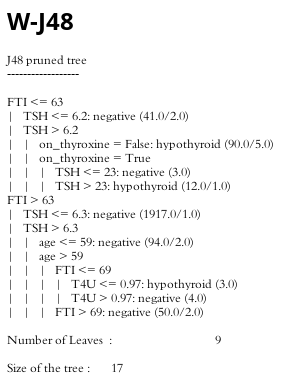
\includegraphics[width=0.35\textwidth]{models/w_j48}
    \caption{Modelo de Árbol generado utilizando el algoritmo C4.5, con una performance de 99.16\%.}
    \label{figure:w_j48}
\end{figure}

En la figura (\ref{figure:w_j48_performance}) se puede observar la performance del modelo obtenido aplicando el mismo sobre un conjunto de testing. \\

\onecolumngrid

\begin{figure*}[ht]
    \centering
    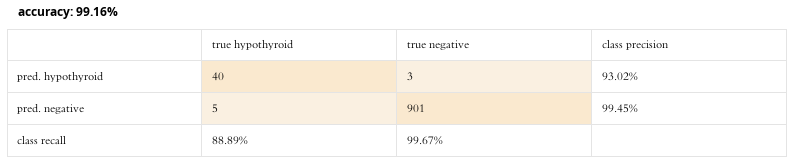
\includegraphics[width=0.75\textwidth]{models/w_j48_performance}
    \caption{Performance del modelo de Árbol generado utilizando el algoritmo C4.5 sobre un conjunto de testeo correspondiente al 30\% del conjunto total de datos.}
    \label{figure:w_j48_performance}
\end{figure*}

\twocolumngrid

\subsection{Reglas de Clasificación}

Para definir el algoritmo a utilizar para la creación de reglas se evalúa cada uno de ellos comparando los modelos generados para determinar así cual es más conveniente. Entre los algoritmos evaluados están OneR y PRISM. \\

\subsubsection{OneR}

Para la construcción de este modelo se trabaja con un conjunto normalizado de los datos utilizando normalización Z sobre los datos de tipo numérico. El antecedente de la regla generada por este algoritmo se define a partir del atributo $FTI$ como se puede observar en la figura (\ref{figure:w_oneR}). \\

\begin{figure}[H]
    \centering
    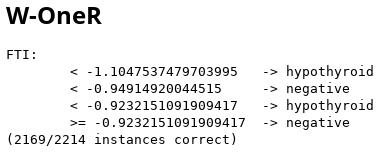
\includegraphics[width=0.4\textwidth]{models/w_oneR}
    \caption{Modelo generado por el algoritmo OneR.}
    \label{figure:w_oneR}
\end{figure}

En la figura (\ref{figure:w_oneR_performance}) se puede observar la performance del modelo obtenido aplicando el mismo sobre un conjunto de testing. \\

\onecolumngrid

\begin{figure*}[ht]
    \centering
    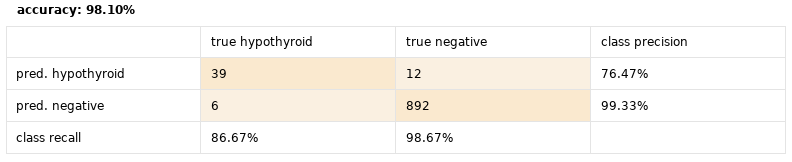
\includegraphics[width=0.75\textwidth]{models/w_oneR_performance}
    \caption{Performance del modelo de reglas generado utilizando el algoritmo OneR sobre un conjunto de testeo correspondiente al 30\% del conjunto total de datos.}
    \label{figure:w_oneR_performance}
\end{figure*}

\twocolumngrid

\subsubsection{PRISM}

Para la construcción del modelo de reglas utilizando el algoritmo PRISM se discretiza por frecuencia los datos numéricos probando le performance del modelo para distintos intervalos. Finalmente se opta por discretizar en 7 intervalos obteniendo los siguientes resultados. \\

\section{Análisis de Resultados}

\section{Discusión y Conclusiones}

\begin{thebibliography}{99}
%% Do not include separate BibTeX files; if BibTeX is used,
%% paste the output (contents of .bbl file) here.

\bibitem{revtex-au} \url{https://authors.aps.org/revtex4/}.
\bibitem{osastyle} \url{http://www.opticsinfobase.org/submit/style/jrnls_style.cfm}.

\end{thebibliography}

\clearpage

\onecolumngrid

\section{Apéndice} 

\subsection{Marco Teórico} \label{apendix:theory}

\subsection{Imágenes} \label{apendix:images}

\subsubsection{Gráficos de los atributos} \label{apendix:images:attr}

\twocolumngrid

\begin{figure}[H]
    \centering
    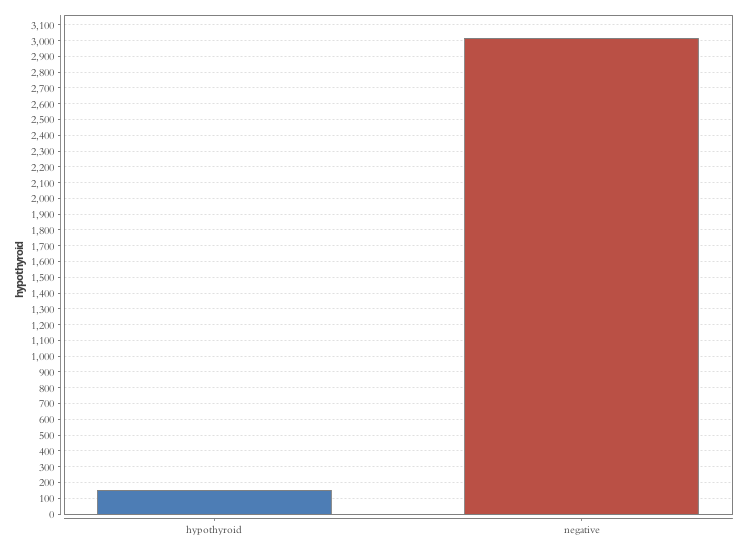
\includegraphics[width=0.45\textwidth]{analysis/bars_hypothyroid}
    \caption{Gráfico de barras del atributo etiqueta.}
    \label{figure:bars_hypothyroid}
\end{figure}

\begin{figure}[H]
    \centering
    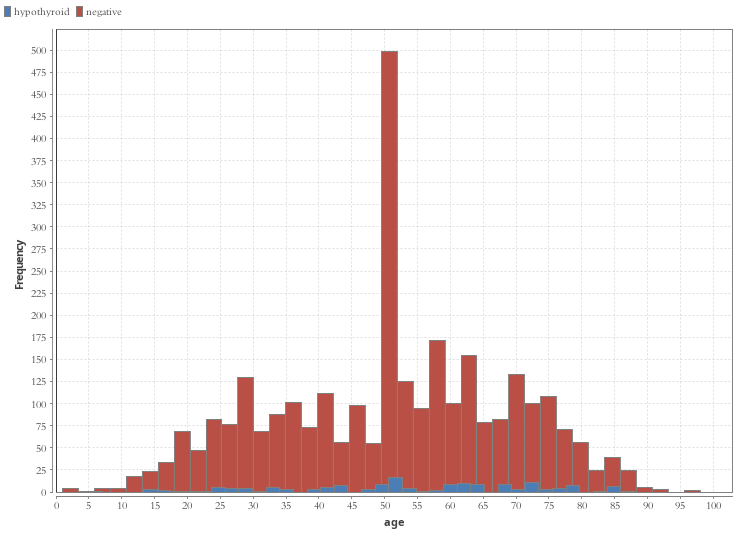
\includegraphics[width=0.45\textwidth]{analysis/histogram_age}
    \caption{Histograma del atributo \textit{age}.}
    \label{figure:histogram_age}
\end{figure}

\begin{figure}[H]
    \centering
    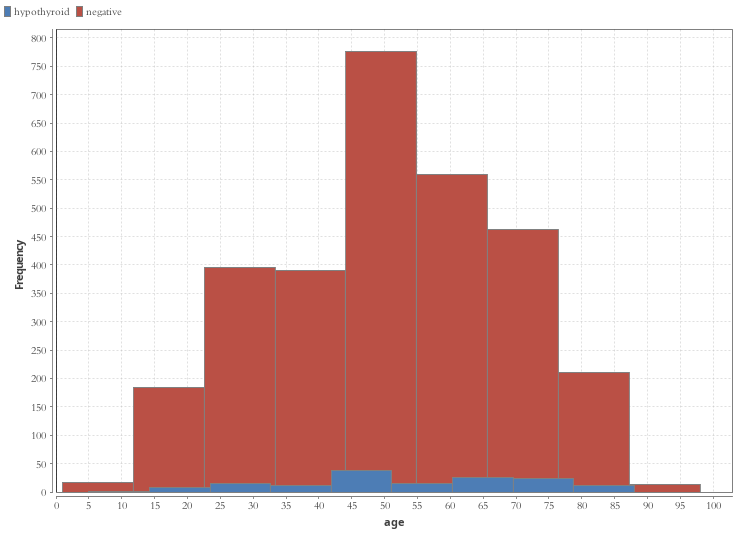
\includegraphics[width=0.45\textwidth]{analysis/histogram_age2}
    \caption{Histograma del atributo \textit{age}.}
    \label{figure:histogram_age2}
\end{figure}

\begin{figure}[H]
    \centering
    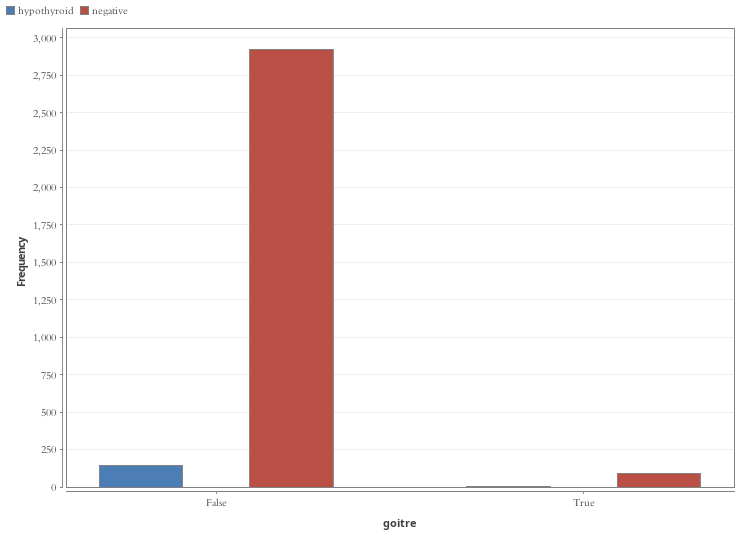
\includegraphics[width=0.45\textwidth]{analysis/histogram_goitre}
    \caption{Histograma del atributo \textit{goitre}.}
    \label{figure:histogram_goitre}
\end{figure}

\begin{figure}[H]
    \centering
    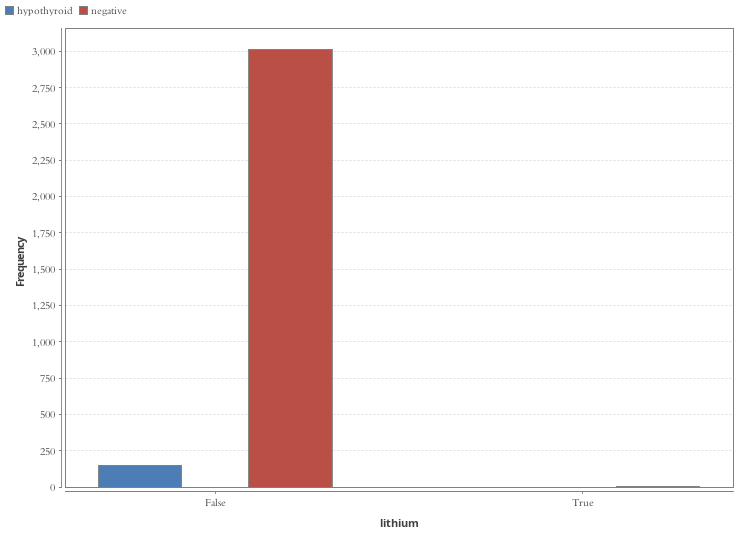
\includegraphics[width=0.45\textwidth]{analysis/histogram_lithium}
    \caption{Histograma del atributo \textit{lithium}.}
    \label{figure:histogram_lithium}
\end{figure}

\begin{figure}[H]
    \centering
    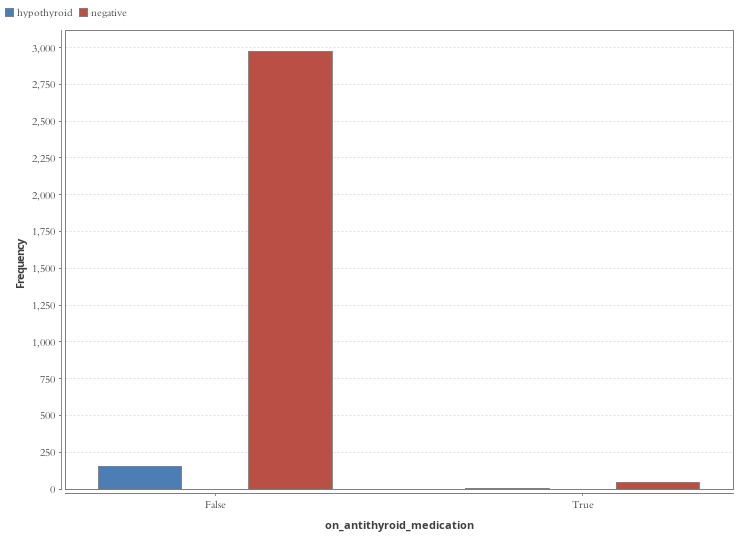
\includegraphics[width=0.45\textwidth]{analysis/histogram_on_antithyroid_medication}
    \caption{Histograma del atributo \textit{on\_antithyroid\_medication}.}
    \label{figure:on_antithyroid_medication}
\end{figure}

\begin{figure}[H]
    \centering
    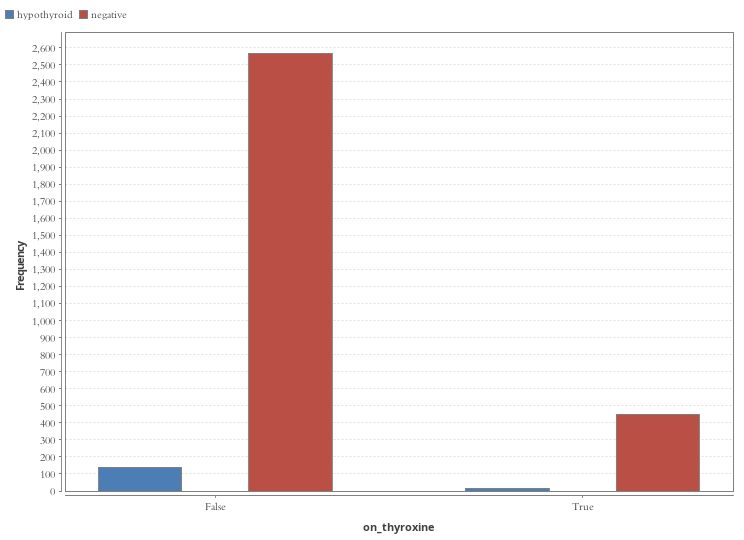
\includegraphics[width=0.45\textwidth]{analysis/histogram_on_thyroxine}
    \caption{Histograma del atributo \textit{on\_thyroxine}.}
    \label{figure:on_thyroxine}
\end{figure}

\begin{figure}[H]
    \centering
    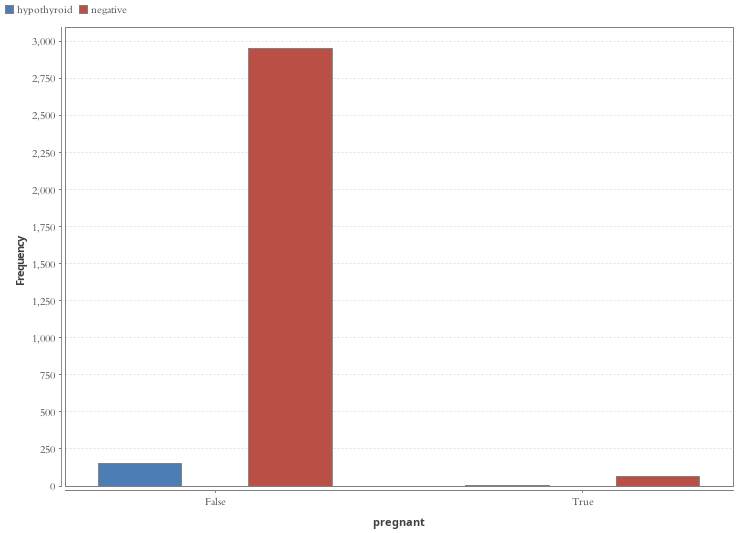
\includegraphics[width=0.45\textwidth]{analysis/histogram_pregnant}
    \caption{Histograma del atributo \textit{pregnant}.}
    \label{figure:pregnant}
\end{figure}

\begin{figure}[H]
    \centering
    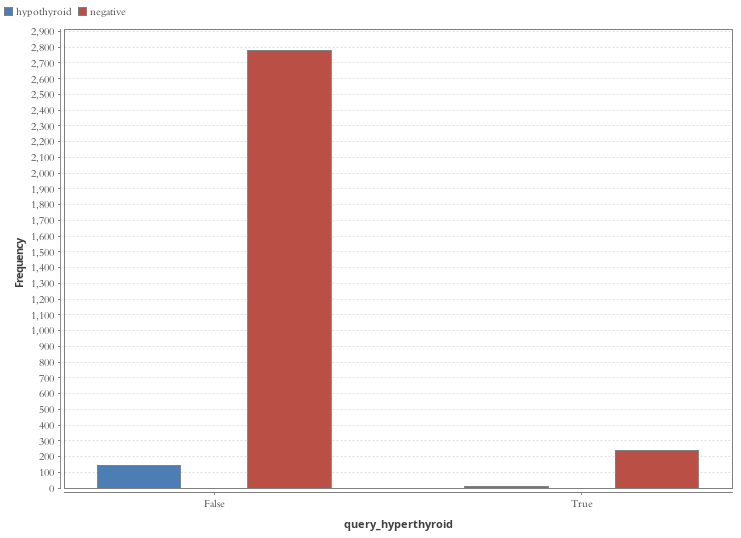
\includegraphics[width=0.45\textwidth]{analysis/histogram_query_hyperthyroid}
    \caption{Histograma del atributo \textit{query\_hyperthyroid}.}
    \label{figure:query_hyperthyroid}
\end{figure}

\begin{figure}[H]
    \centering
    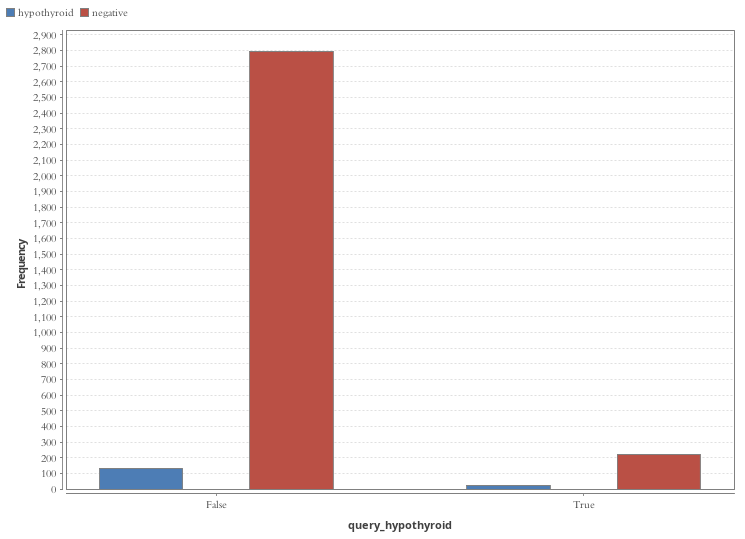
\includegraphics[width=0.45\textwidth]{analysis/histogram_query_hypothyroid}
    \caption{Histograma del atributo \textit{query\_hypothyroid}.}
    \label{figure:query_hypothyroid}
\end{figure}

\begin{figure}[H]
    \centering
    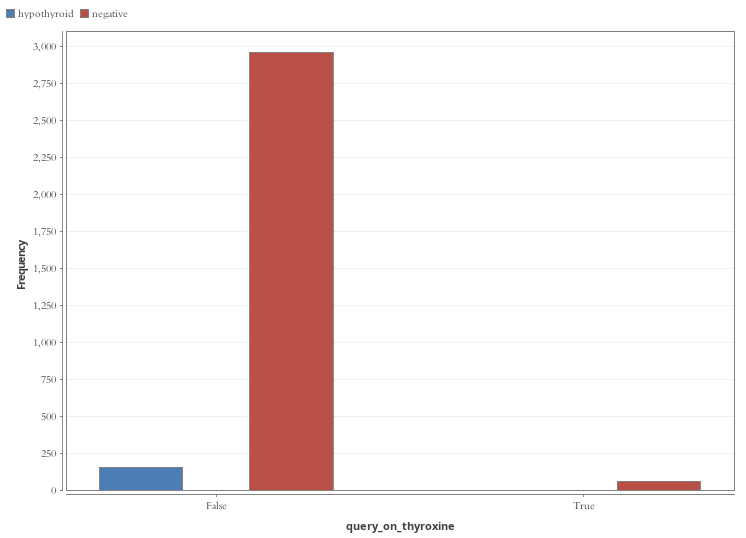
\includegraphics[width=0.45\textwidth]{analysis/histogram_query_on_thyroxine}
    \caption{Histograma del atributo \textit{query\_on\_thyroxine}.}
    \label{figure:query_on_thyroxine}
\end{figure}

\begin{figure}[H]
    \centering
    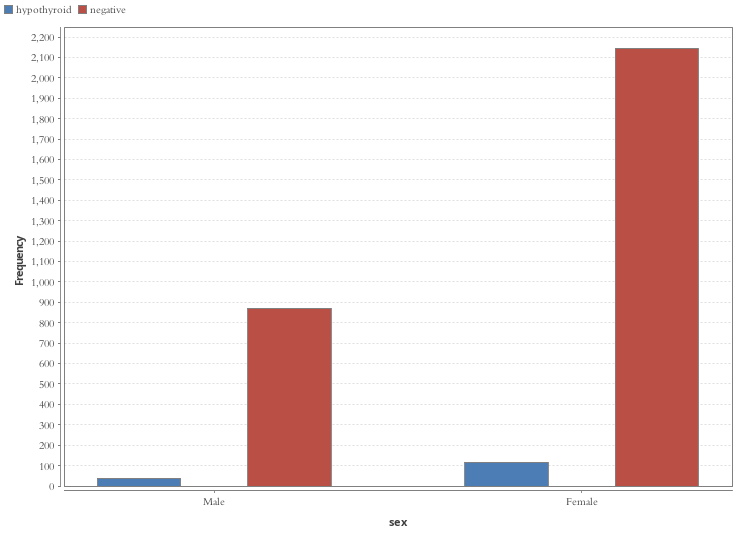
\includegraphics[width=0.45\textwidth]{analysis/histogram_sex}
    \caption{Histograma del atributo \textit{sex}.}
    \label{figure:sex}
\end{figure}

\begin{figure}[H]
    \centering
    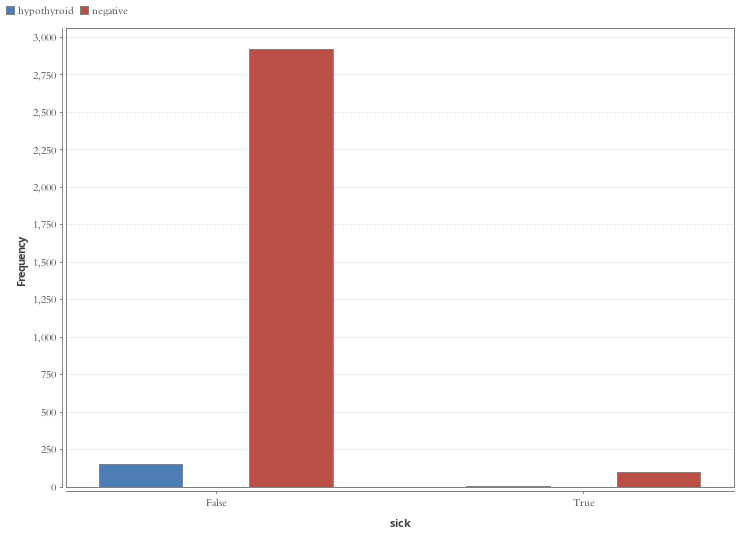
\includegraphics[width=0.45\textwidth]{analysis/histogram_sick}
    \caption{Histograma del atributo \textit{sick}.}
    \label{figure:sick}
\end{figure}

\begin{figure}[H]
    \centering
    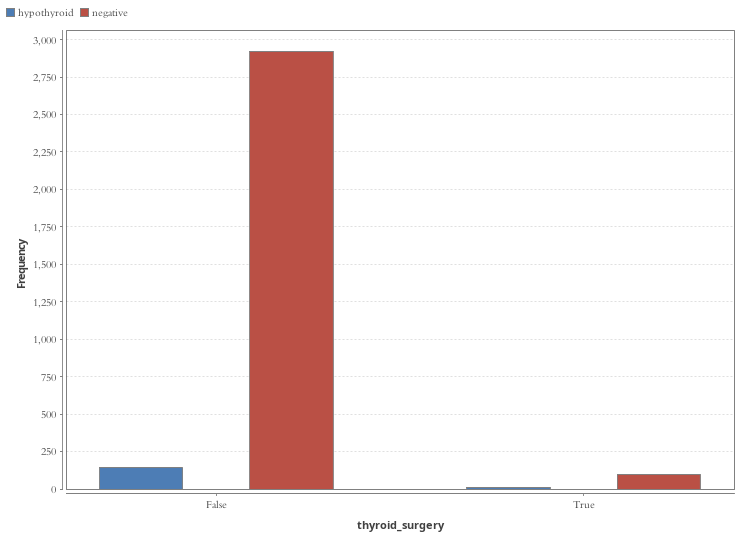
\includegraphics[width=0.45\textwidth]{analysis/histogram_thyroid_surgery}
    \caption{Histograma del atributo \textit{thyroid\_surgery}.}
    \label{figure:thyroid_surgery}
\end{figure}

\begin{figure}[H]
    \centering
    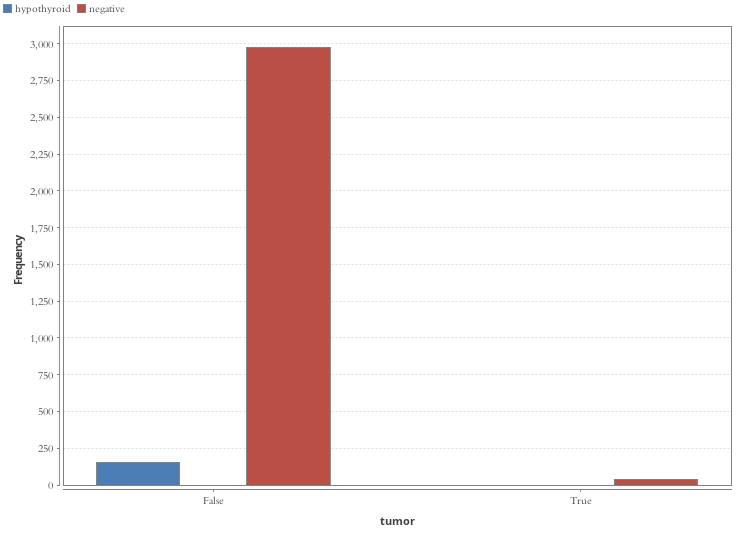
\includegraphics[width=0.45\textwidth]{analysis/histogram_tumor}
    \caption{Histograma del atributo \textit{tumor}.}
    \label{figure:tumor}
\end{figure}

\begin{figure}[H]
    \centering
    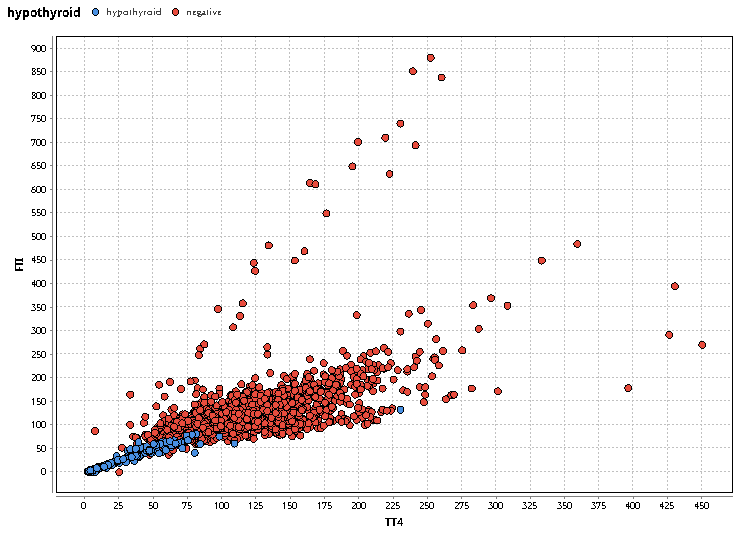
\includegraphics[width=0.45\textwidth]{analysis/scatter_TT4_FTI}
    \caption{Diagrama de dispersión de los atributos \textit{TT4, FTI}.}
    \label{figure:scatter_TT4_FTI}
\end{figure}

\begin{figure}[H]
    \centering
    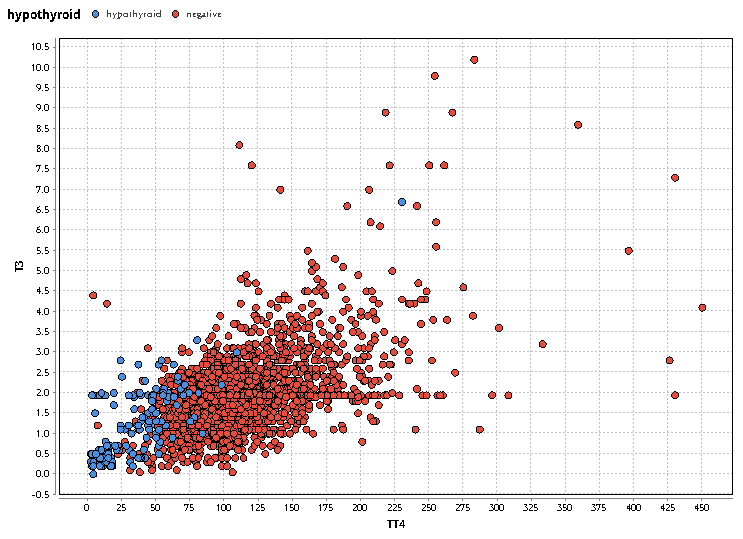
\includegraphics[width=0.45\textwidth]{analysis/scatter_TT4_T3}
    \caption{Diagrama de dispersión de los atributos \textit{TT4, T3}.}
    \label{figure:scatter_TT4_T3}
\end{figure}

\begin{figure}[H]
    \centering
    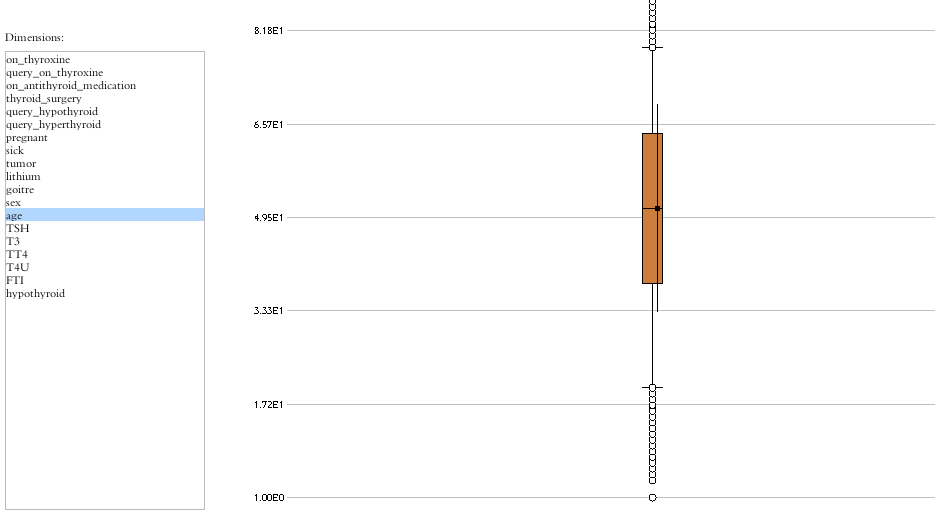
\includegraphics[width=0.45\textwidth]{analysis/box_plot_age}
    \caption{Diagrama de cajas del atributo \textit{age}.}
    \label{figure:box_plot_age}
\end{figure}

\begin{figure}[H]
    \centering
    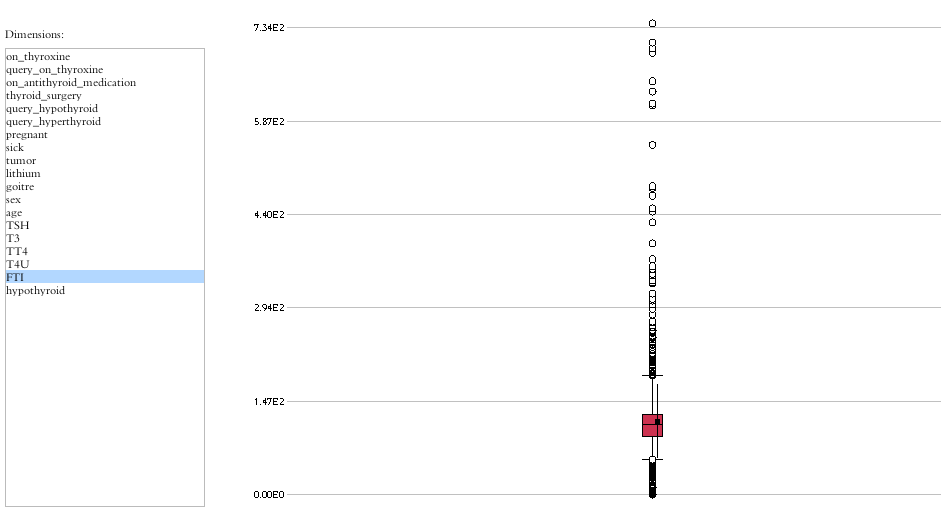
\includegraphics[width=0.45\textwidth]{analysis/box_plot_FTI}
    \caption{Diagrama de cajas del atributo \textit{FTI}.}
    \label{figure:box_plot_FTI}
\end{figure}

\begin{figure}[H]
    \centering
    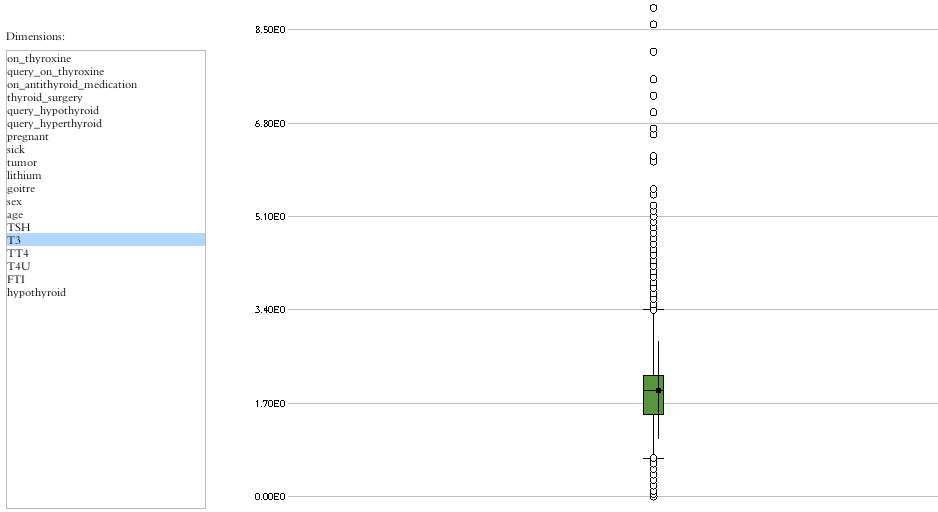
\includegraphics[width=0.45\textwidth]{analysis/box_plot_T3}
    \caption{Diagrama de cajas del atributo \textit{T3}.}
    \label{figure:box_plot_T3}
\end{figure}

\begin{figure}[H]
    \centering
    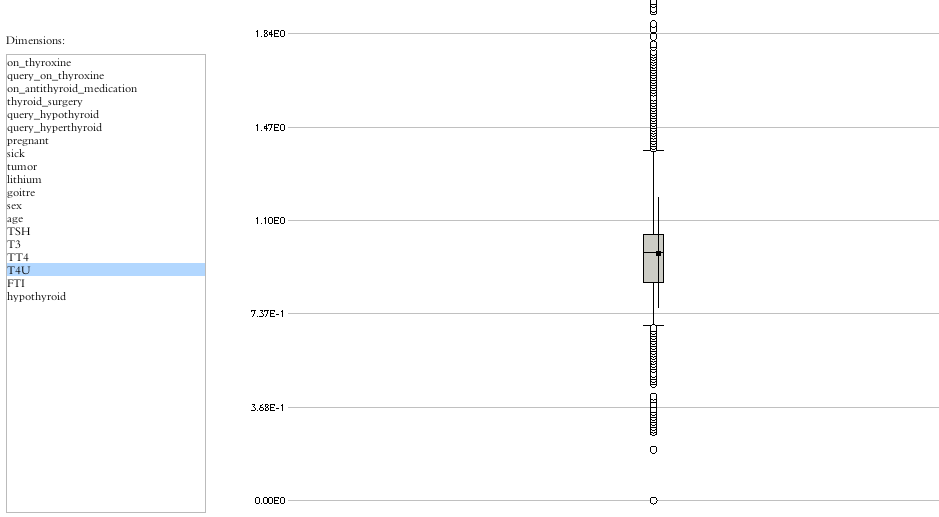
\includegraphics[width=0.45\textwidth]{analysis/box_plot_T4U}
    \caption{Diagrama de cajas del atributo \textit{T4U}.}
    \label{figure:box_plot_T4U}
\end{figure}

\begin{figure}[H]
    \centering
    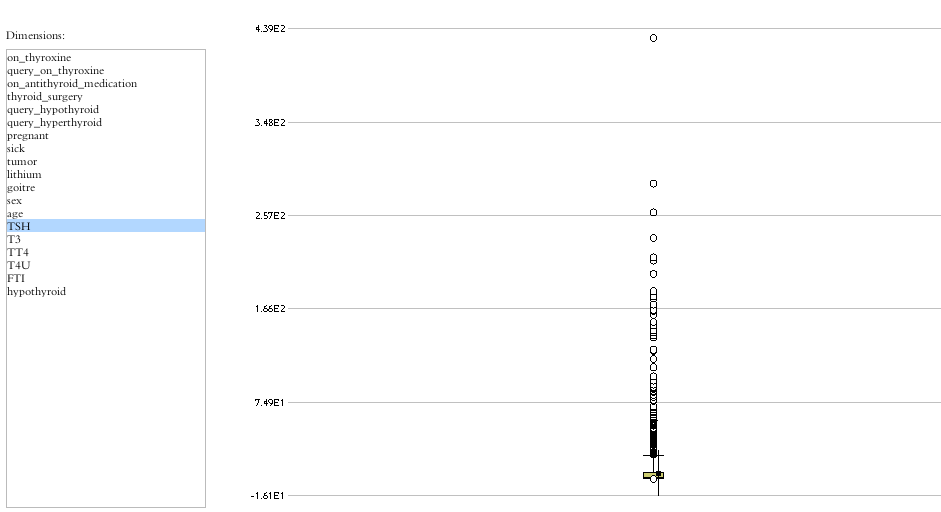
\includegraphics[width=0.45\textwidth]{analysis/box_plot_TSH}
    \caption{Diagrama de cajas del atributo \textit{TSH}.}
    \label{figure:box_plot_TSH}
\end{figure}

\onecolumngrid



\end{document}
